% Welcome! This is the unofficial University of Udine beamer template.

% See README.md for more informations about this template.

% This style has been developed following the "Manuale di Stile"
% (Style Manual) of the University of Udine. You can find the
% manual here: https://www.uniud.it/it/ateneo-uniud/ateneo-uniud/identita-visiva/manuali-immagine-stile/manuale-stile

% Note: for some reason, the RGB values specified in the manual
% do NOT render correctly in Beamer, so they have been redefined
% for this document using the high level chromo-optic deep neural 
% quantistic technology offered by Microsoft Paint's color picker.

% We defined four theme colors: UniBrown, UniBlue, UniGold
% and UniOrange. For example, to write some uniud-brownish
% text, just use: \textcolor{UniBrown}{Hello!}

% Note that [usenames,dvipsnames] is MANDATORY due to compatibility
% issues between tikz and xcolor packages.

\documentclass[usenames,dvipsnames,table]{beamer}
\usepackage[utf8]{inputenc}
\usepackage{verbatim}
\usetheme{uniud}


%%% Bibliography
\usepackage[
  backend=biber,
  style=numeric,
  citestyle=numeric,
  giveninits=true,
  eprint=false,
  url=false,
  doi=false,
  isbn=false
]{biblatex}
\addbibresource{bibliography.bib}

% Author names in publication list are consistent 
% i.e. name1 surname1, name2 surname2
% See https://tex.stackexchange.com/questions/106914/biblatex-does-not-reverse-the-first-and-last-names-of-the-second-author
\DeclareNameAlias{author}{given-family}

%%% Suppress biblatex annoying warning
\usepackage{silence}
\WarningFilter{biblatex}{Patching footnotes failed}

%%% Some useful commands
% pdf-friendly newline in links
\newcommand{\pdfnewline}{\texorpdfstring{\newline}{ }} 
% Fill the vertical space in a slide (to put text at the bottom)
\newcommand{\framefill}{\vskip0pt plus 1filll}


\title[University of Udine]{\LARGE Comparison of Tools for the Verification of Cryptographic Protocols}
\date[September 2021]{\small September 21, 2021}
\author[Alessandro Zanatta]{\small Alessandro Zanatta}
\institute{\small Course in Computer Network Security}

%% -------------------------------------------------------------------------------- %%
%% Additional packages                                                              %% 
%% -------------------------------------------------------------------------------- %%
\usepackage{listings}
\usepackage{cleveref}
\usepackage{afterpage}
\usepackage{msc}
\usepackage[euler]{textgreek}
\usepackage[justification=centering]{caption}
\usepackage{courier}
\usepackage{tikz}
\usepackage{array}
\usepackage{pifont}
\usepackage{multirow}
\usepackage{ctable}
\usepackage{booktabs}
\usepackage{changepage}
\usepackage{caption}
\usepackage{soul}
\usepackage{multicol}

\graphicspath{{logos/},{images/}} % Images folder(s)

\captionsetup[table]{name=}
\captionsetup[figure]{name=}
\renewcommand{\lstlistingname}{}
\captionsetup{skip=5pt,font=scriptsize,labelfont=scriptsize}

\setbeamercolor{alerted text}{fg=white}
\sethlcolor{UniOrange}
\renewcommand<>{\hl}[1]{\only#2{\beameroriginal{\hl}}{#1}}
\makeatletter
\let\HL\hl
\renewcommand\hl{%
  \let\set@color\beamerorig@set@color
  \let\reset@color\beamerorig@reset@color
  \HL}
\makeatother
\SoulColor

\setbeamercovered{transparent}

%% -------------------------------------------------------------------------------- %%
%% Commands                                                                         %%
%% -------------------------------------------------------------------------------- %%

% Highlight text
\newcommand<>{\myhl}[1]{\alert#2{\hl#2{#1}}}

% Checkmark and cross
\newcommand{\cmark}{\ding{51}}
\newcommand{\xmark}{\ding{55}}

% Basic setting for listings
\lstset{basicstyle=\scriptsize\ttfamily,breaklines=true,captionpos=b}

% msc options command
\newcommand\setmscoptions{%
  \setlength{\instdist}{1.5cm}%
  % \setlength{\levelheight}{1.5 \levelheight}%
  % \setlength{\instwidth}{3cm}
  \setmsckeyword{}
  \drawframe{no}
  \centering
}

\newcommand*{\Z}{\ensuremath{\mathbb{Z}}}
\newcommand*{\Q}{\ensuremath{\mathbb{Q}}}

%% Taken from https://hal.inria.fr/file/index/docid/955869/filename/sapic.tex
\newcommand{\msrewrite}[1]{\mathrel{-\hspace{-2pt}[#1]\hspace{-4pt}\to}}
\newcommand{\emptyrule}{\ensuremath{[]}\xspace}
\newcommand{\msr}[3]{\ensuremath{\left[#1\right] \msrewrite{#2} \left[#3\right]}}
%% -------------- %%

\newcommand{\msrfact}[2]{\ensuremath{\mbox{#1}\left(#2\right)}}

% Multiset rewriting rules
\newcommand{\msrnolabel}[2]{\ensuremath{#1 \rightarrow #2}}
\newcommand{\msrsetminus}{\ensuremath{\setminus^\#}}
\newcommand{\msrcap}{\ensuremath{\cap^\#}}
\newcommand{\msrcup}{\ensuremath{\cup^\#}}
\newcommand{\msrin}{\ensuremath{\in^\#}}
\newcommand{\msrsubseteq}{\ensuremath{\subseteq^\#}}

% Applied pi-calculus
\newcommand{\pic}{\textpi-calculus }
\newcommand{\picnospace}{\textpi-calculus}

% Cryptographic primitives
\newcommand{\func}[2]{\ensuremath{\mbox{#1}\left(#2\right)}}
\newcommand{\enc}[2]{\ensuremath{\left\{#1\right\}_{#2}}}
\newcommand{\sha}[2]{\ensuremath{\func{sha#1}{#2}}}
\newcommand{\kdf}[1]{\ensuremath{\func{kdf}{#1}}}
\newcommand{\fpk}[1]{\ensuremath{\func{fpk}{#1}}}
\newcommand{\hash}[1]{\ensuremath{\func{hash}{#1}}}
\newcommand{\modexp}[3]{\ensuremath{#1^#2 \mod{#3}}}
\newcommand{\key}[1]{\ensuremath{k_{#1}}}
\newcommand{\pkey}[1]{\ensuremath{pk_{#1}}}
\newcommand{\skey}[1]{\ensuremath{sk_{#1}}}
\newcommand{\newkey}[1]{\ensuremath{k'_{#1}}}
\newcommand{\group}[1]{\ensuremath{\Z_{#1}}}

% Circles
\newcommand*\emptycirc[1][1ex]{\tikz\draw[] (0,0) circle (#1);} 
\newcommand*\halfcirc[1][1ex]{%
  \begin{tikzpicture}
  \draw[fill] (0,0)-- (90:#1) arc (90:270:#1) -- cycle ;
  \draw (0,0) circle (#1);
  \end{tikzpicture}}
\newcommand*\fullcirc[1][1ex]{\tikz\fill (0,0) circle (#1);} 

% Multiline comments
\renewcommand{\comment}[1]{}

%% -------------------------------------------------------------------------------- %%
%% Languages listings                                                               %%
%% -------------------------------------------------------------------------------- %%
\lstdefinelanguage{tamarin}
{
  keywordstyle=\color{MidnightBlue}\bfseries,
  keywordstyle=[2]\itshape,
  keywordstyle=[3]\color{Green}\bfseries,
  keywordstyle=[4]\color{RedViolet}\bfseries,
  keywords={let, in, Out, In, K, KU, Fr},
  keywords=[2]{},
  keywords=[3]{},
  keywords=[4]{rule},
  sensitive=true,
  morecomment=[l]{//},
  morecomment=[n][\color{OliveGreen}\itshape]{/*}{*/},
  morestring=[b]",
}

\lstdefinelanguage{verifpal}
{
  keywordstyle=\color{MidnightBlue}\bfseries,
  keywordstyle=[2]\itshape,
  keywordstyle=[3]\color{Green}\bfseries,
  keywordstyle=[4]\color{Orange}\bfseries,
  alsoletter={->, ?},
  keywords={principal, attacker, queries, ->, ?, ASSERT, PKE_DEC, PKE_ENC},
  keywords=[2]{Client, Server, Alice, Bob},
  keywords=[3]{leaks, phase},
  keywords=[4]{active, passive},
  sensitive=true,
  morecomment=[l]{//}
}

\lstdefinelanguage{proverif}
{
  keywordstyle=\color{MidnightBlue}\bfseries,
  keywordstyle=[2]\itshape,
  keywordstyle=[3]\color{Green}\bfseries,
  keywords={table, query, insert, leaks, phase, get, out, event, in, ., ;, attacker, |, new, if, else, then, !, let},
  alsoletter={., ;, |, !},
  keywords=[2]{Client, Server},
  keywords=[3]{},
  sensitive=true,
  morecomment=[l]{//},
  morecomment=[n][\color{OliveGreen}\itshape]{(*}{*)},
  morestring=[b]",
}


% Bibliography size
\renewcommand*{\bibfont}{\scriptsize}

%% -------------------------------------------------------------------------------- %%
%% Start of beamer document                                                         %%
%% -------------------------------------------------------------------------------- %%

\begin{document}

\begin{frame}
  \titlepage
\end{frame}

\begin{frame}{Outline}
  \footnotesize
  \tableofcontents
\end{frame}

\section{Why?}
\begin{frame}[t]{Why?}
  Cryptographic protocols are:
  \begin{itemize}
    \item{ubiquitous;}\pause
    \item{fundamental for security;}\pause
    \item{error-prone (e.g. Needham-Schroeder Public Key \cite{NSPK} and Lowe fix \cite{NSLPK}).}
  \end{itemize}

  \vskip 1cm

  \onslide<3->{Solution?}

  \onslide<4>{\begin{center}
      \LARGE\textbf{\textcolor{UniGold}{Formal verification of protocols!}}\par
    \end{center}}

\end{frame}

\section{How?}
\begin{frame}[t]{How?}
  Two possible models:
  \begin{itemize}
    \pause
    \item{\myhl<3->{Symbolic model};}
    \item{Computational model.}
  \end{itemize}

  \vskip 0.5cm

  \pause\pause
  Main elements:
  \begin{itemize}
    \pause
    \item{Attacker $\to$ Dolev-Yao \cite{DolevYao};}\pause
    \item{Cryptographic primitives $\to$ black-box;}\pause
    \item{Messages $\to$ terms.}\pause
    \item{\myhl{Perfect cryptography} assumption;}
  \end{itemize}

  \vskip 0.5cm
\end{frame}

\begin{frame}[t]{Perfect cryptography assumption example}

  Suppose we have:
  \begin{itemize}
    \pause
    \item{Two primitives: $\mbox{enc}$, $\mbox{dec}$;}\pause
    \item{Two terms: $m$, $k$;}\pause
    \item{The following equality:
                \begin{equation}
                  \mbox{dec}\left(\mbox{enc}\left(m, k\right), k\right) = m
                \end{equation}
          }
  \end{itemize}

  \vskip 0.5cm

  \onslide<5>{
    Under the \textcolor{UniGold}{perfect cryptography} assumption:
    \begin{center}
      can decrypt $\mbox{enc}\left(m, k\right) \Longleftrightarrow k$ is known
    \end{center}}
\end{frame}

\begin{frame}[t]{Available tools}
  Many automatic tools:
  \begin{itemize}
    \item{\myhl<2->{Tamarin prover}}
    \item{\myhl<2->{Proverif}}
    \item{\myhl<2->{Verifpal}}
    \item{Scyther}
    \item{Scyther-proof}
    \item{AVISPA project}
    \item{Maude NPA}
    \item{... and others}
  \end{itemize}
\end{frame}

\section{Tamarin prover, Proverif and Verifpal}
\framecard{Tamarin prover,\\Proverif and Verifpal}

\subsection{Tamarin prover}
\begin{frame}{Tamarin prover}
  Based on \cite{TamarinFoundations,TamarinManual}:
  \begin{itemize}
    \item{Protocol and adversary capabilities $\to$ \myhl<5->{Labelled multiset rewriting rules};}\pause
    \item{Security properties $\to$ Guarded fragment of first order logic (with timepoints);}\pause
    \item{Cryptographic primitives $\to$ Functions and equational theories;}\pause
    \item{Verification $\to$ Constraint solving algorithm (backward-search and heuristics).}
  \end{itemize}
\end{frame}

\begin{frame}[fragile]{Labelled multiset rewriting rules}
  \lstset{language=tamarin}
  \begin{itemize}
    \item{Terms $\to$ can be thought of as messages;}
    \item{Facts $\to$ model information;}
    \item{Special facts $\to$ \lstinline{In(x)}, \lstinline{Out(x)}, \lstinline{Fr(x)} and \lstinline{K(x)};}
    \item{State $\to$ Multiset of facts;}
    \item{Transition rules $\to$ allows transitions between states.
                \begin{lstlisting}
rule ExampleRule:
    [ PremiseFact(x) ]
  --[ ActionFact(x)]->
    [ ConclusionFact(x) ]
    \end{lstlisting}}
    \item{Trace $\to$ sequence of (ground) facts.}
  \end{itemize}
\end{frame}

\begin{frame}{State transitions}
  \begin{block}{State transitions}
    Consider a ground multiset rewriting rule $\msr{l}{a}{r}$.

    If we call the state of the system $S$, the trace $T$ and assuming $l \msrsubseteq S$, the new state $S'$ is defined as:
    \begin{equation}
      S' = S \msrsetminus l \msrcup r
    \end{equation}
    Additionally, we append $a$ to the end of the current trace.
  \end{block}
\end{frame}

\subsection{Proverif}
\begin{frame}{Proverif}
  Based on \cite{ProverifFoundations}:
  \begin{itemize}
    \item{Protocol and adversary capabilities $\to$ \myhl<5->{\hbox{Applied \picnospace}};}\pause
    \item{Security properties $\to$ Queries on events (Horn clauses);}\pause
    \item{Cryptographic primitives $\to$ Constructors, destructors and equations;}\pause
    \item{Verification $\to$ Resolution algorithm applied on the protocol translation to Horn clauses.}
  \end{itemize}
\end{frame}

\comment{
\begin{frame}{Proverif II}
  \begin{figure}
    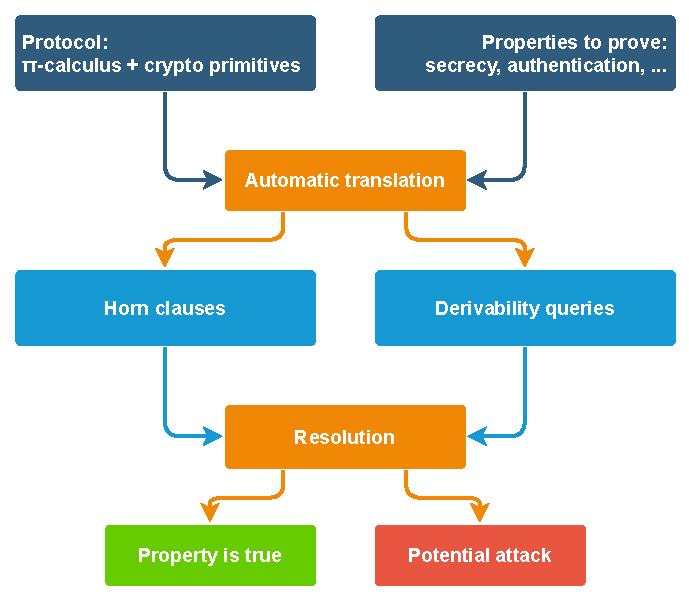
\includegraphics[scale=0.7]{proverif-verification-method}
    \caption{Proverif's verification method.}
  \end{figure}
\end{frame}
}

\begin{frame}[fragile]{Proverif's applied \picnospace}
  \lstset{language=proverif}
  Grammar of processes ($P$, $Q$):
  \begin{lstlisting}
0                    (* null process *)
out(N, M); P         (* output to channel N the message M *)
in(N, M: T); P       (* input from channel N of message M *)
P | Q                (* parallel composition *)
!P                   (* infinite replication *)
new a: T; P          (* fresh value of sort T *)
if M then P else Q   (* conditional *)
  \end{lstlisting}
  \vskip 0.5cm
  Additionally:
  \begin{lstlisting}
event EventName(x);        (* add event to trace *)
query event(EventName(x)). (* define a query on events *)
phase t;                   (* execute a process in phase t *)
let macroName = P.         (* create a process macro *)
let x = M in P else Q.     (* assignment and pattern matching *)
  \end{lstlisting}
\end{frame}

\subsection{Verifpal}
\begin{frame}{Verifpal}
  \lstset{language=verifpal,basicstyle=\footnotesize\ttfamily}
  Based on \cite{VerifpalManual,VerifpalFoundations}:
  \begin{itemize}
    \item Protocol and adversary capabilities $\to$ \lstinline{principal} blocks and message exchanges;\pause
    \item Security properties $\to$ \lstinline{queries} block;\pause
    \item Cryptographic primitives $\to$ pre-defined (no user-defined ones);\pause
    \item Verification $\to$ Custom resolution algorithm.
          % in slide \ref{frame:verifpal-res-alg}.
  \end{itemize}
\end{frame}

\begin{frame}[t,fragile]{Verifpal}
  Verifpal minimal working example:
  \lstset{language=verifpal,basicstyle=\scriptsize\ttfamily}
  \begin{lstlisting}
attacker [active]

principal Alice [ knows private x ]
Alice -> Bob: x
principal Bob []

queries []
  \end{lstlisting}
  \pause
  \lstset{language=verifpal,basicstyle=\footnotesize\ttfamily}
  Constructs:
  \begin{itemize}
    \item{\lstinline{attacker} $\to$ \lstinline{active} or \lstinline{passive};}\pause
    \item{Inside a \lstinline{principal} block:
                \begin{itemize}
                  \item{\lstinline{generates}, \lstinline{knows}, \lstinline{leaks}}
                  \item{assignments}
                  \item{cryptographic primitives}
                \end{itemize}
          }\pause
    \item{\lstinline{queries} $\to$ confidentiality, authentication, freshness, unlinkability and equivalence.}
  \end{itemize}
\end{frame}

% \begin{frame}[label={frame:verifpal-res-alg}]{Resolution steps}
%   \begin{figure}
%     \vspace*{-0.2cm}
%     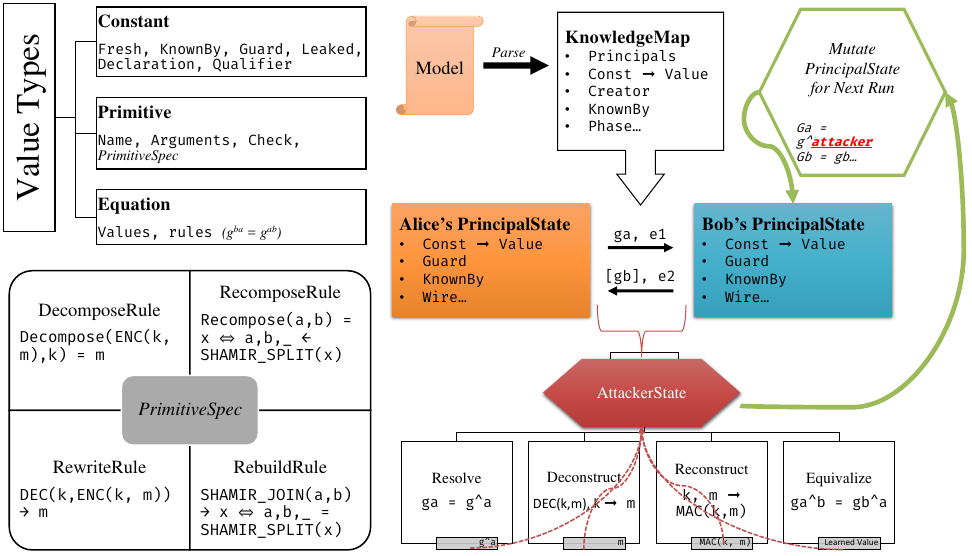
\includegraphics[scale=.35]{verifpal-internals}
%     \caption{All credits to Nadim Kobeissi.}
%   \end{figure}
%   \vspace*{-0.8cm}
%   \begin{multicols}{2}
%     \begin{enumerate}
%       \item{Gather values;}
%       \item{Populate attacker state;}
%       \item{Apply transformations;}
%       \item{Prepare next mutations;}
%       \item{Mutate protocol executions.}
%     \end{enumerate}
%   \end{multicols}
% \end{frame}

\section{Case studies}
\framecard[UniBlue]{Case studies:\\Diffie-Hellman and\\Needham-Schroeder Public Key}

\begin{frame}{Case studies}
  Two case studies:
  \begin{itemize}
    \item{Diffie-Hellman}
    \item{Needham-Schroeder Public Key}
  \end{itemize}

  \vskip 1cm

  \begin{block}{Source code}
    The source code of the case studies is available on github \cite{CaseStudies}.
  \end{block}
\end{frame}

\subsection{Diffie-Hellman}
\begin{frame}[fragile]{Diffie-Hellman}
  \begin{columns}[c]
    \column{0.6\textwidth}
    We will consider three versions:
    \begin{itemize}
      \item{Anonymous}
      \item{Ephemeral}
      \item{Post-Compromise Ephemeral}
    \end{itemize}
    \column{0.4\textwidth}
    \begin{figure}[t]
      \setmscoptions
      \begin{msc}{}
        \setmscscale{.5}

        \declinst{client}{}{Client}
        \declinst{server}{}{Server}

        \action*{\parbox{3.5cm}{\centering
            Knows $g, p$\\
            $c \in \Z$\\
            $g_c := \modexp{g}{c}{p}$
          }}{client}

        \nextlevel[5]
        \mess{$g_c$}{client}{server}
        \nextlevel

        \action*{\parbox{3.5cm}{\centering
            Knows $g, p$\\
            $s \in \Z$\\
            $g_s := \modexp{g}{s}{p}$\\
            $\skey{c} := \modexp{g_c}{s}{p}$
          }}{server}

        \nextlevel[6]
        \mess{$g_s$}{server}{client}
        \nextlevel

        \action*{\parbox{3.5cm}{\centering
            $\key{cs} := \modexp{g_s}{c}{p}$
          }}{client}
        \nextlevel

      \end{msc}
      \centering
    \end{figure}
  \end{columns}
\end{frame}

% \begin{frame}[fragile]{Anonymous Diffie-Hellman}
%   Straightforward implementation.

%   \vskip 0.25cm

%   To store keys (for message exchanges):
%   \begin{itemize}
%     \lstset{language=tamarin}
%     \item{Tamarin $\to$ Persistent fact: \lstinline{!ClientKey(k)}}
%     \lstset{language=proverif}
%     \visible<2->{\item{Proverif $\to$ Table: \lstinline{insert ClientKeyTable(k);}}}
%   \end{itemize}

%   \lstset{basicstyle=\scriptsize\ttfamily}
%   \begin{columns}[onlytextwidth,t]
%     \hspace*{-.60cm}
%     \begin{column}{0.5\paperwidth}
%       \centering
%       \lstset{language=tamarin}
%       \begin{lstlisting}[caption=Tamarin]
% /* Send a message from client to server */
% rule ClientSendMessage:
%     [
%       Fr(~m),
%       !ClientKey(k)
%     ]
%   --[ ClientSentMessage(k, ~m) ]->
%     [ Out(senc(<'CtoS', ~m>, k)) ]
%       \end{lstlisting}
%     \end{column}

%     \begin{column}{0.5\paperwidth}

%       \begin{onlyenv}<2->
%         \centering
%         \lstset{language=proverif}
%         \begin{lstlisting}[caption=Proverif]
% let ClientSendsMessage() =
%   (* Generate fresh message m *)
%   new m: Plaintext;

%   (* Get client key from table *)
%   get ClientKey(k) in
%   event ClientSentMessage(m, k);
%   out(io, enc(m, k));
%   0.
%       \end{lstlisting}
%       \end{onlyenv}
%     \end{column}
%   \end{columns}
% \end{frame}

% \begin{frame}[fragile]{Ephemeral Diffie-Hellman}
%   Server half key needs to be authenticated:
%   \begin{itemize}
%     \item{Tamarin $\to$ private channel with passive attacker:
%                 \begin{lstlisting}[language=tamarin]
% rule CertificateExchange:
%     [ CertificateOut(x) ] --> [ CertificateIn(x), Out(x) ]
%       \end{lstlisting}
%           }\pause
%     \item{Proverif $\to$ table (output every value we insert):
%                 \begin{lstlisting}[language=proverif]
% table AuthenticatedValueTable(G).

% let Server() =
%   ...
%   insert AuthenticatedValueTable(g_r);
%   out(io, g_r);
% ...
%     \end{lstlisting}
%           }\pause
%     \item{Verifpal $\to$ guarded variables (between square brackets):
%                 \begin{lstlisting}[language=verifpal]
% Server -> Client: [g_s], c1
%     \end{lstlisting}
%           }
%   \end{itemize}
% \end{frame}

% \begin{frame}[t,fragile]{Post-Compromise Ephemeral DH I}
%   We model the leakage of ephemeral keys:
%   \begin{itemize}
%     \item{Tamarin $\to$ Fact for the ephemeral key, rule to output it:
%                 \begin{lstlisting}[language=tamarin]
% rule RevealClientEphemeralKey:
%     [ ClientEphemeralKey(c) ]
%   --[ RevealedClientEphemeralKey(c) ]->
%     [ Out(c) ]
%       \end{lstlisting}
%                 Use lemma timepoints to leak the value after a certain action fact;
%           }\pause
%     \lstset{language=proverif}
%     \item{Proverif $\to$ create a process in \lstinline{phase 1}:
%                 \begin{lstlisting}
% let PostRevealClientEphemeralKey =
%   phase 1;
%   (* Get the client's ephemeral key and output it *)
%   get ClientEphemeralKeyTable(c) in
%   out(io, c);
%   event PostRevealedClientEphemeralKeyTable(c);
%   0.
%     \end{lstlisting}
%           }
%   \end{itemize}
% \end{frame}

% \begin{frame}[t,fragile]{Post-Compromise Ephemeral DH II}
%   \lstset{language=verifpal}
%   \begin{itemize}
%     \item{Verifpal $\to$ very similar to Proverif, using \lstinline{phase} and \lstinline{leaks}:
%     \begin{lstlisting}
% phase [1]

% principal Client [
%   leaks c
% ]

% principal Server [
%   leaks s
% ]
% \end{lstlisting}
%     }
%   \end{itemize}
% \end{frame}

\subsection{Needham-Schroeder Public Key}
\begin{frame}[t]{Needham-Schroeder Public Key}
  \begin{columns}[T]
    \column{0.6\textwidth}
    We will consider two versions of the (simplified) Needham-Schroeder Public Key protocol:
    \begin{itemize}
      \item{Flawed}
      \item{Fixed: message 2 is changed from $\enc{NA, NB}{\pkey{A}}$ to $\enc{B, NA, NB}{\pkey{A}}$.}
    \end{itemize}
    \column{0.4\textwidth}
    \begin{figure}
      \vspace*{-1cm}
      \setmscoptions
      \setlength{\instdist}{2cm}
      \begin{msc}{}
        \setmscscale{.5}

        \declinst{alice}{}{Alice}
        \declinst{bob}{}{Bob}

        \action*{\parbox{3.5cm}{\centering
            Knows $\skey{A}, \pkey{A}$\\
            Knows $\pkey{B}$
          }}{alice}

        \action*{\parbox{3.5cm}{\centering
            Knows $\skey{B}, \pkey{B}$\\
            Knows $\pkey{A}$
          }}{bob}
        \nextlevel[4]

        \action*{\parbox{3.5cm}{\centering
            Generates $N_A$
          }}{alice}

        \nextlevel[3]
        \mess{$\enc{N_A, A}{\pkey{B}}$}{alice}{bob}
        \nextlevel


        \action*{\parbox{3.5cm}{\centering
            Generates $N_B$
          }}{bob}

        \nextlevel[3]
        \mess{$\enc{N_A, N_B}{\pkey{A}}$}{bob}{alice}
        \nextlevel[2]
        \mess{$\enc{N_B}{\pkey{B}}$}{alice}{bob}

      \end{msc}
    \end{figure}
  \end{columns}
  \begin{block}{Important modelling trick}
    We need to allow the attacker to decide with whom the initiator executes the protocol.
  \end{block}
\end{frame}

% \begin{frame}[t,fragile]{Flawed NSPK protocol I}
%   Modelling attacker deciding responder:
%   \begin{itemize}
%     \item{Tamarin $\to$ we fix the initiator as Alice (i.e. the attacker chooses only the responder):
%                 \begin{lstlisting}[language=tamarin]
% rule 1_Initiator:
%   let I = 'Alice' in
%     [        
%       /* Responder identity */
%       In(R),
%       /* Get public key of responder */
%       !PublicKey(R, pk_R),
%       ...
%     ]
%   --[...]->
%     [...]
%       \end{lstlisting}
%                 Two rules are used to create the persistent fact for key pairs of both honest parties and attacker;
%           }
%   \end{itemize}
% \end{frame}
% \begin{frame}[t,fragile]{Flawed NSPK protocol II}
%   \begin{itemize}
%     \item{Proverif $\to$ in Proverif we let the attacker decide every participant identity:
%                 \begin{lstlisting}[language=proverif]
% let Initiator() =
%   (* Attacker sends communicating parties *)
%   in(io, (X: Principal, rUser: Principal));

%   (* We restrict them: X must be honest and they must differ *)
%   let iUser = isHonest(X, Alice, Bob) in
%   if iUser <> rUser then

%   (* Get private key of initiator *)
%   get PrivateKeyTable(=iUser, skI) in

%   (* Get public key of responder *)
%   get PublicKeyTable(=rUser, pkR) in
%   ...
%       \end{lstlisting}
%                 Similar to Tamarin, two processes create key pairs for honest parties and the attacker;
%           }
%   \end{itemize}
% \end{frame}
% \begin{frame}[t,fragile]{Flawed NSPK protocol III}
%   \begin{itemize}
%     \item{Verifpal $\to$ straightforward implementation, with a caveut. We need to pre-share public keys and responder's one must be unguarded.
%                 \begin{lstlisting}[language=verifpal]
% Alice -> Bob: [K_PA]
% Bob -> Alice: K_PB
% \end{lstlisting}
%                 This allows the attacker to mutate Bob's public key to its own, initiating the MITM.
%           }
%   \end{itemize}
% \end{frame}

% \begin{frame}{Fixed NSPK protocol}
%   No changes, apart from the protocol fix.
% \end{frame}

\subsection{Results}
\begin{frame}{Results}
  \begin{overlayarea}{\textwidth}{\textheight}
    \begin{overlayarea}{\textwidth}{.3\textheight}
      Same results with (almost) every tool!
      \vspace*{-0.5cm}
      \begin{columns}[t]
        \begin{column}{0.5\textwidth}
          \begin{table}
            \renewcommand{\arraystretch}{1.4}
            \rowcolors{2}{gray!25}{white}
            \setlength\arrayrulewidth{1pt}
            \makebox[\textwidth][c]{
              \scalebox{0.6}{
                \begin{tabular}{c|cc}
                  \multicolumn{1}{l|}{}    & \textbf{Secrecy} & \textbf{Authentication} \\ \hline
                  \textbf{Anonymous}       & \xmark           & \xmark                  \\
                  \textbf{Ephemeral}       & Client to server & Server to client        \\
                  \textbf{Post-compromise} & \xmark           & Server to client
                \end{tabular}
              }
            }
            \caption{Diffie-Hellman}
          \end{table}
        \end{column}

        \begin{column}{0.5\textwidth}
          \begin{table}
            \renewcommand{\arraystretch}{1.4}
            \rowcolors{2}{gray!25}{white}
            \setlength\arrayrulewidth{1pt}
            \makebox[\textwidth][c]{
              \scalebox{0.6}{
                \begin{tabular}{c|cc}
                  \multicolumn{1}{l|}{} & \textbf{Nonces secrecy} & \textbf{Authentication} \\ \hline
                  \textbf{Flawed}       & \xmark                  & \xmark                  \\
                  \textbf{Fixed}        & \cmark                  & \cmark                  \\
                \end{tabular}
              }
            }
            \caption{Needham-Schroeder Public Key}
          \end{table}
        \end{column}
      \end{columns}
    \end{overlayarea}

    \begin{overlayarea}{\textwidth}{.7\textheight}
      \only<2>{
        \begin{figure}
          \centering
          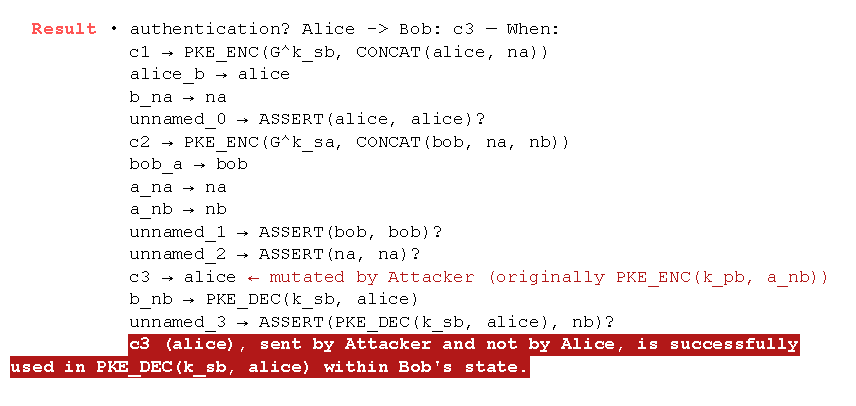
\includegraphics[scale=.7]{verifpal-nspk-trace}
        \end{figure}
      }
      \only<3>{
        \begin{block}{Mail from Nadim Kobeissi}
          ``This analysis result appears to be completely correct to me. The
          ASSERT call occurs after Bob decrypts enca. So yes, the protocol does not finish
          its run, but Bob still manages to use the non-authentic enca before the protocol
          is aborted! Hence the result.''
        \end{block}
      }
    \end{overlayarea}
  \end{overlayarea}
\end{frame}

\section{Tools comparison}
\framecard[UniBrown]{Tools comparison}

\begin{frame}{Tools comparison}
  Five metrics:
  \begin{itemize}
    \item Usability;
    \item Expressiveness;
    \item Efficiency;
    \item Soundness;
    \item Completeness.
  \end{itemize}
\end{frame}

\subsection{Usability}
\begin{frame}[t]{Usability I}
  Usability as:
  \begin{columns}[t]
    \begin{column}{0.6\textwidth}
      \begin{itemize}
        \item{Easiness of modeling:
                    \begin{enumerate}
                      \item<2->{Verifpal
                                  \begin{itemize}
                                    \item simple and intuitive language;
                                    \item offers a very useful VS-Code extension;
                                  \end{itemize}
                            }
                      \item<3->{Proverif
                                  \begin{itemize}
                                    \item steep learning curve;
                                    \item challenging constructs to grasp;
                                  \end{itemize}
                            }
                      \item<4->{Tamarin
                                  \begin{itemize}
                                    \item very steep learning curve;
                                    \item challenging constructs to grasp;
                                  \end{itemize}
                            }
                    \end{enumerate}}
      \end{itemize}
    \end{column}
    \begin{column}{0.4\textwidth}
      \only<2->{
        \begin{figure}
          \vspace*{-1.6cm}
          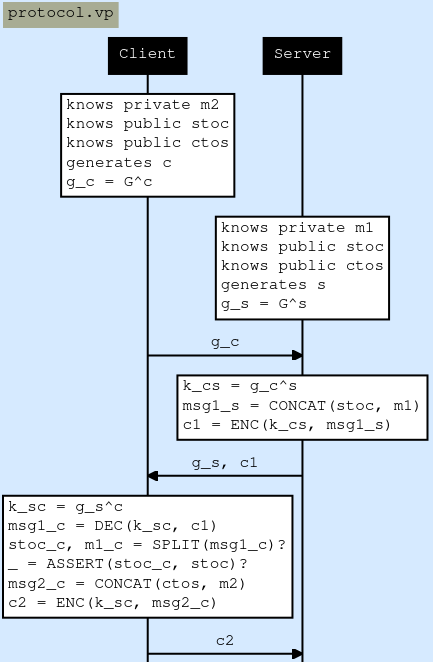
\includegraphics[scale=.38]{verifpal-protocol-graph}
          \caption{Verifpal model graph in VS-Code}
        \end{figure}
      }
    \end{column}
  \end{columns}
\end{frame}

\begin{frame}[t]{Usability II}
  \begin{itemize}
    \item{Attack traces visualization:
                \begin{itemize}
                  \item<only@1> Textual
                  \item<only@2> Graph view (only Tamarin and Proverif)
                \end{itemize}
          }
  \end{itemize}

  \begin{figure}
    \vspace*{-0.3cm}
    \includegraphics<1>[scale=.4]
    {attack-trace-comparison}
  \end{figure}
  \vspace*{-1.6cm}
  \only<2>{
    \begin{columns}
      \begin{column}{0.4\textwidth}
        \begin{figure}
          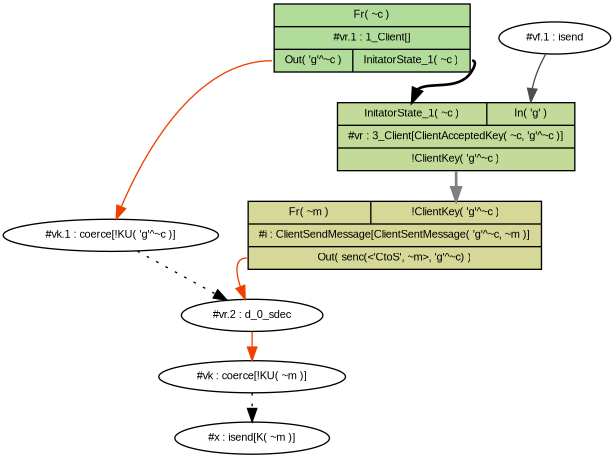
\includegraphics[scale=.35]{tamarin-trace}
          \caption{Tamarin trace}
        \end{figure}
      \end{column}
      \begin{column}{0.6\textwidth}
        \begin{figure}
          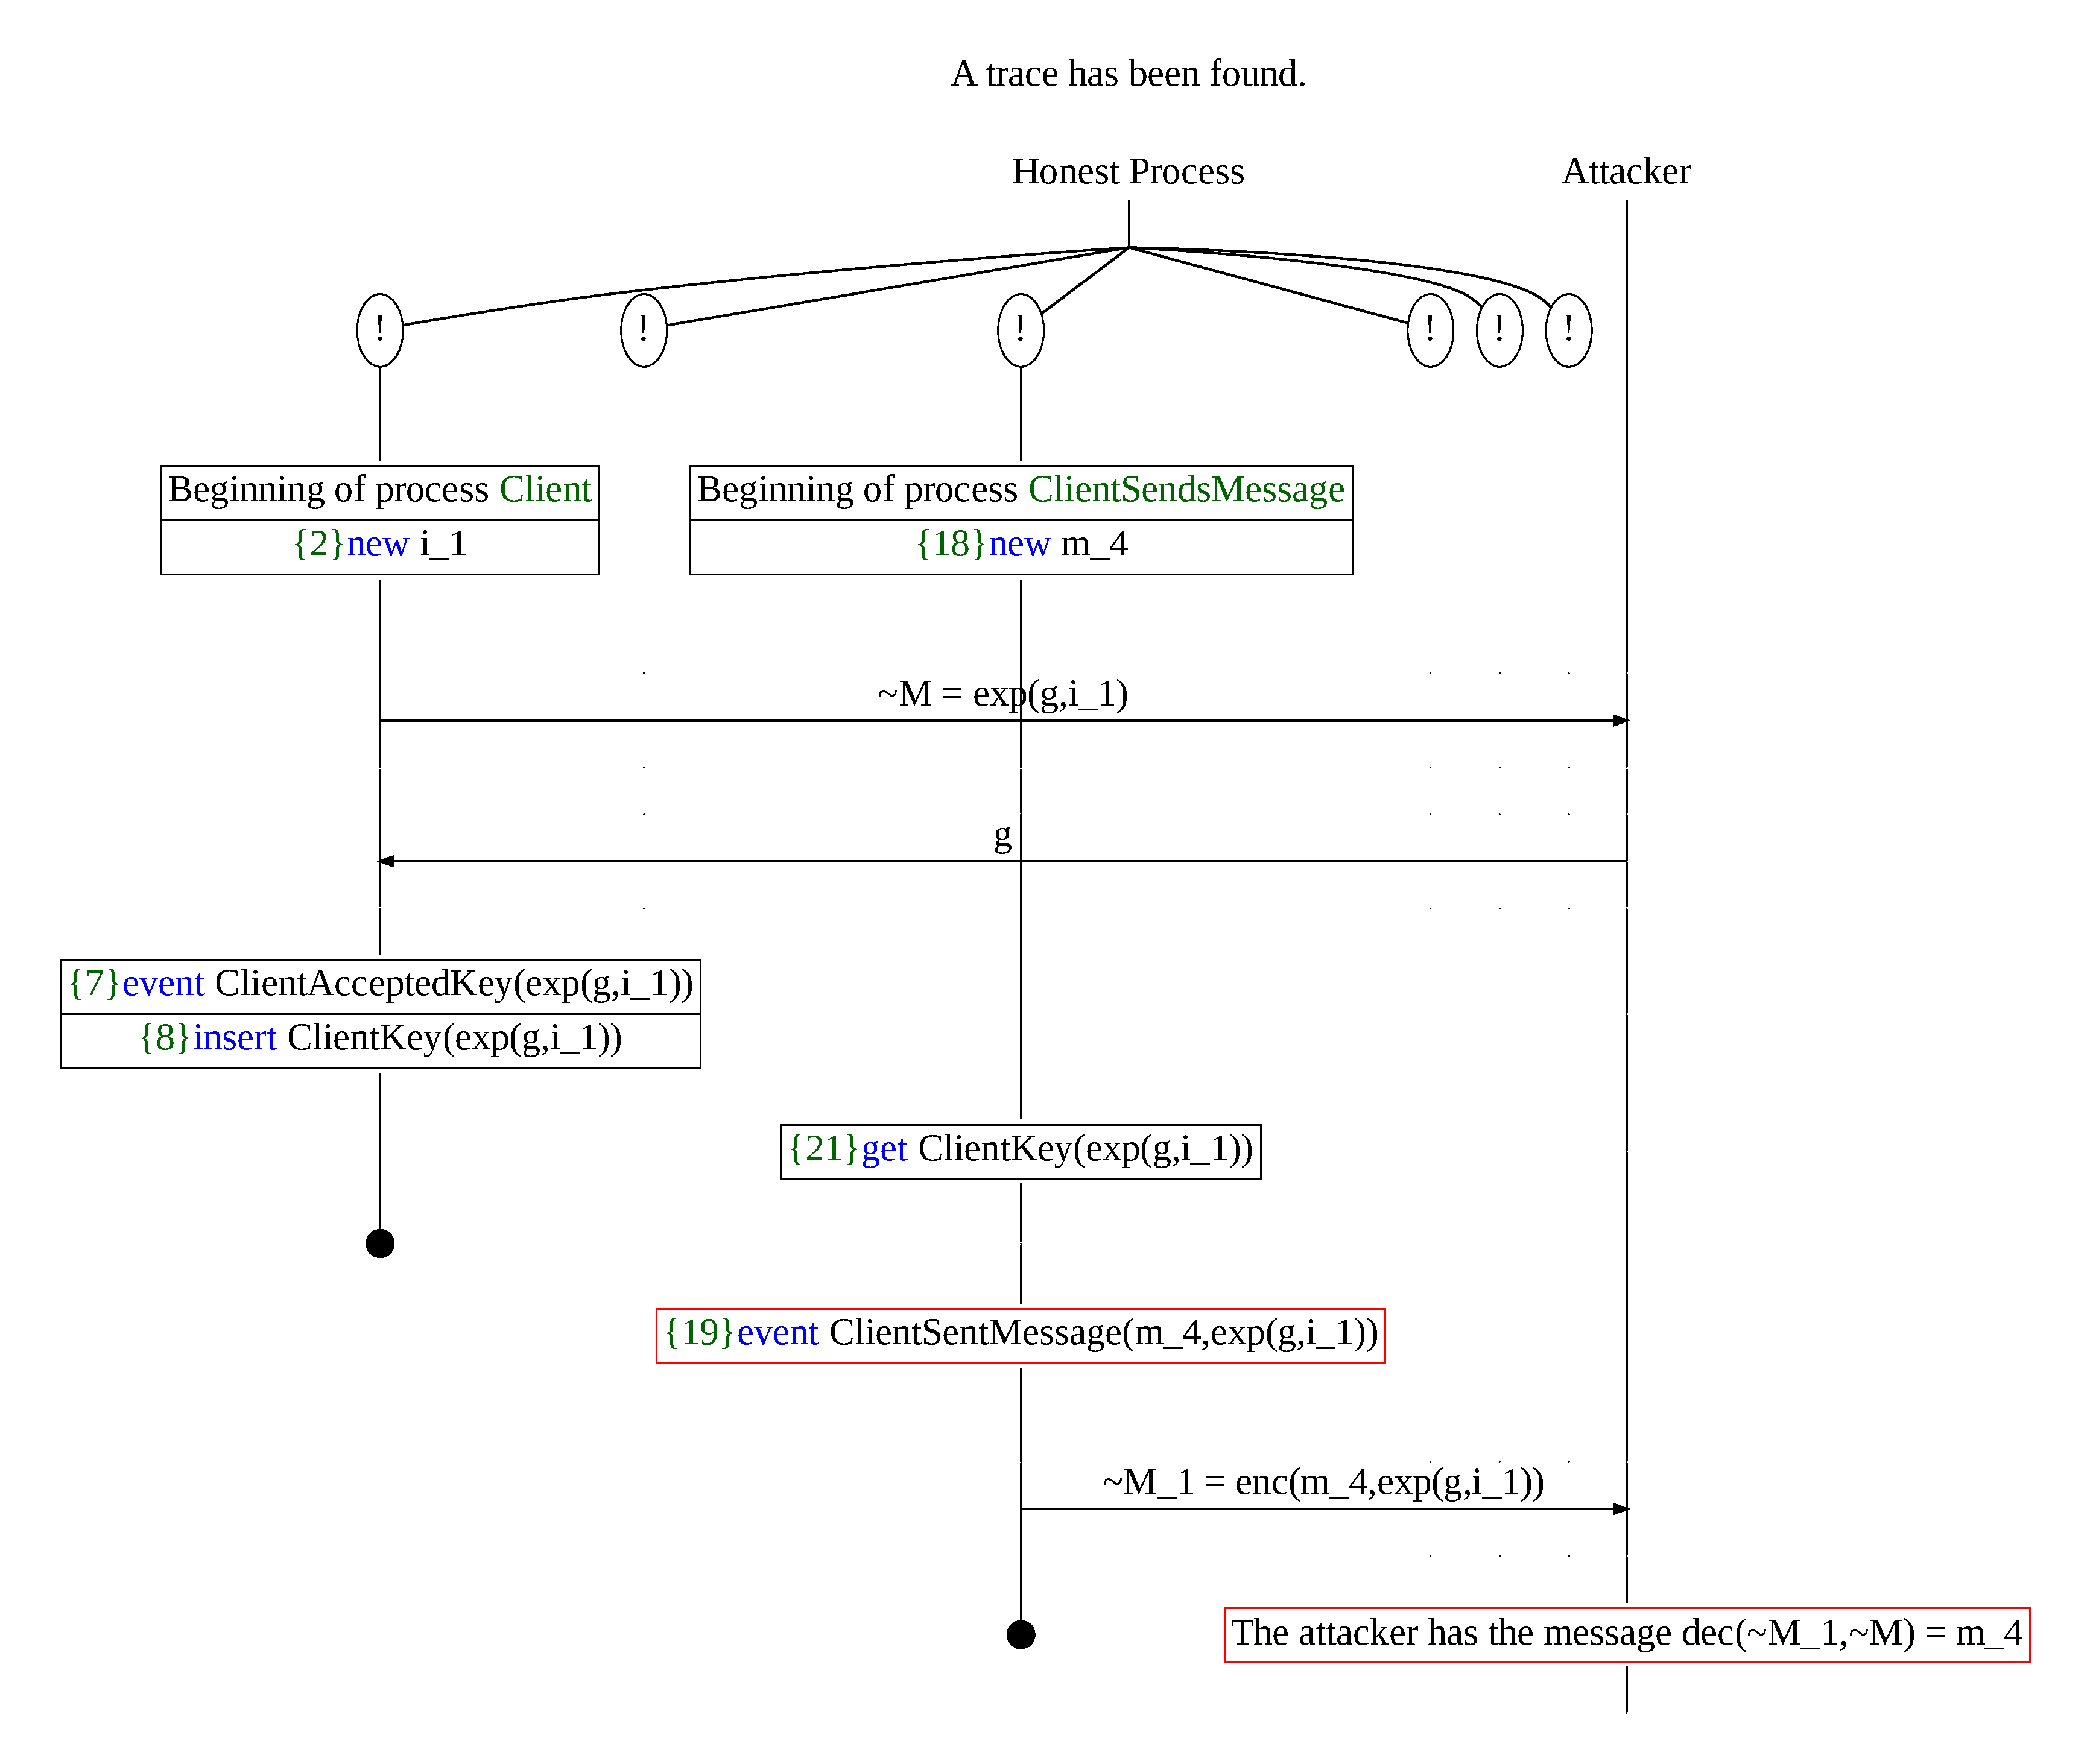
\includegraphics[scale=.12]{proverif-trace}
          \caption{Proverif trace}
        \end{figure}
      \end{column}
    \end{columns}
  }
\end{frame}


\subsection{Expressiveness}
\begin{frame}{Expressiveness}
  \vskip 0.5cm
  \begin{overlayarea}{\textwidth}{\textheight}
    \begin{overlayarea}{\textwidth}{.3\textheight}
      \begin{table}[!ht]
        \renewcommand{\arraystretch}{1.5}
        \setlength\arrayrulewidth{1pt}
        \rowcolors{2}{gray!25}{white}
        \makebox[\textwidth][c]{
          \scalebox{0.8}{
            \begin{tabular}{c|ccccc}
              \multicolumn{1}{l|}{} & \textbf{Unbounded} & \textbf{Equational theory} & \textbf{State} & \textbf{Obs. Equiv.} & \textbf{Linkability} \\ \hline
              \textbf{Tamarin}      & \fullcirc          & \fullcirc                  & \fullcirc      & \fullcirc            & \emptycirc           \\
              \textbf{Proverif}     & \fullcirc          & \halfcirc                  & \halfcirc      & \fullcirc            & \emptycirc           \\
              \textbf{Verifpal}     & \fullcirc          & \halfcirc                  & \fullcirc      & \emptycirc           & \fullcirc
            \end{tabular}
          }
        }
      \end{table}
    \end{overlayarea}

    \only<2>{
      \begin{overlayarea}{\textwidth}{.7\textheight}
        \begin{block}{Observational equivalence}
          Two systems appear the same to the environment. \textit{or}
          Two entities are indistinguishable on the basis of their observable implications.
        \end{block}
      \end{overlayarea}
    }

    \only<3>{
      \begin{overlayarea}{\textwidth}{.7\textheight}
        \begin{block}{Linkability}
          Following Verifpal's definition:
          ``For two observed values, the adversary cannot distinguish between a protocol execution in which they belong to the same user and a protocol execution in which they belong to two different users''
        \end{block}
      \end{overlayarea}
    }
  \end{overlayarea}

\end{frame}

\subsection{Efficiency}
\begin{frame}[t]{Efficiency}
  \vspace*{-0.5cm}
  
\begin{table}[!ht]
\caption{Comparison table for Diffie-Hellman.}
\label{tab:DH}
\setlength\arrayrulewidth{1pt}
\rowcolors{2}{gray!25}{white}
\makebox[\textwidth][c]{
    \scalebox{0.9}{
    \begin{tabular}{c|ccc|ccc|ccc|l}
    \cline{2-10}
    \multicolumn{1}{l|}{} & \multicolumn{3}{c|}{\textbf{Peak memory size (kb)}} & \multicolumn{3}{c|}{\textbf{Time (s)}} & \multicolumn{3}{c|}{\textbf{CPU time}} &  \\ \cline{2-10}
    \multicolumn{1}{l|}{}                    & Tamarin & Verifpal & Proverif & Tamarin & Verifpal & Proverif & Tamarin & Verifpal & Proverif & \\ \hline
    \multicolumn{1}{c|}{Mean}      & 52445 & 11480 & 10639 & 1136 & 13  & 44  & 3.52 & 2.08 & 0.98 & \multicolumn{1}{c}{} \\ \cline{1-10}
    \multicolumn{1}{c|}{Deviation} & 2541  & 244   & 108   & 106  & 1   & 1   & 0.06 & 0.12 & 0.02 & \multicolumn{1}{c}{} \\ \cline{1-10}
    \multicolumn{1}{c|}{Median}    & 52120 & 11464 & 10616 & 1125 & 12  & 44  & 3.52 & 2.08 & 0.97 & \multicolumn{1}{c}{\parbox[t]{1em}{\multirow{-3}{*}{\rotatebox[origin=c]{90}{\textbf{Anon}}}}} \\ \hline
    
    \multicolumn{1}{c|}{Mean}      & 39731 & 13112 & 10623 & 841  & 67  & 34  & 3.38 & 3.24 & 0.98 & \multicolumn{1}{c}{} \\ \cline{1-10}
    \multicolumn{1}{c|}{Deviation} & 1824  & 257   & 110   & 106  & 7   & 0   & 0.04 & 0.06 & 0.02 & \multicolumn{1}{c}{} \\ \cline{1-10}
    \multicolumn{1}{c|}{Median}    & 39742 & 13008 & 10604 & 814  & 72  & 34  & 3.38 & 3.25 & 0.97 & \multicolumn{1}{c}{\parbox[t]{1em}{\multirow{-3}{*}{\rotatebox[origin=c]{90}{\textbf{Eph}}}}} \\ \hline

    \multicolumn{1}{c|}{Mean}      & 44273 & 13098 & 11112 & 1312 & 75 & 81 & 3.47 & 3.14 & 0.98 & \multicolumn{1}{c}{} \\ \cline{1-10}
    \multicolumn{1}{c|}{Deviation} & 1518  & 250   & 112   & 201  & 8  & 1  & 0.04 & 0.10 & 0.01 & \multicolumn{1}{c}{} \\ \cline{1-10}
    \multicolumn{1}{c|}{Median}    & 43914 & 12994 & 11092 & 1319 & 80 & 81 & 3.48 & 3.16 & 0.98 & \multicolumn{1}{c}{\parbox[t]{1em}{\multirow{-3}{*}{\rotatebox[origin=c]{90}{\textbf{PFS}}}}} \\
    \end{tabular}
    }
}
\end{table}\pause
  \vspace*{-1.2cm}
  
\begin{table}[!ht]
\caption{Comparison table for Needham-Schroeder Public Key.}
\label{tab:NSPK}
\makebox[\textwidth][c]{
    \begin{tabular}{c|c|c|c|c|c|c|c|c|c|l}
    \cline{2-10}
    \multicolumn{1}{l|}{} & \multicolumn{3}{c|}{\textbf{Peak memory size (kb)}} & \multicolumn{3}{c|}{\textbf{Time (s)}} & \multicolumn{3}{c|}{\textbf{CPU time}} &  \\ \cline{2-10}
    \multicolumn{1}{l|}{}                    & Tamarin & Verifpal & Proverif & Tamarin & Verifpal & Proverif & Tamarin & Verifpal & Proverif & \\ \hline
    \multicolumn{1}{|c|}{Mean} & 59803 & 13286 & 11106 & 3336 & 40 & 86 & 3.70 & 2.05    & 0.99 & \multicolumn{1}{l|}{\parbox[t]{1em}{\multirow{3}{*}{\rotatebox[origin=c]{90}{\textbf{Flawed}}}}} \\ \cline{1-10}
    \multicolumn{1}{|c|}{Deviation} & 2860 & 317 & 107 & 188 & 4 & 1 & 0.05 & 0.05 & 0.01 & \multicolumn{1}{l|}{} \\ \cline{1-10}
    \multicolumn{1}{|c|}{Median}    & 59498 & 13224 & 11088 & 3345 & 40 & 86 & 3.70 & 2.05 & 0.98 & \multicolumn{1}{l|}{} \\ \specialrule{.2em}{0em}{0em}

    \multicolumn{1}{|c|}{Mean}      & 53217 & NA & 10698 & 1929 & NA & 69 & 3.63 & NA    & 0.99 & \multicolumn{1}{l|}{\parbox[t]{1em}{\multirow{3}{*}{\rotatebox[origin=c]{90}{\textbf{Fixed}}}}} \\ \cline{1-10}
    \multicolumn{1}{|c|}{Deviation} & 2802 & NA & 109 & 164 & NA & 1 & 0.05 & NA & 0.01 & \multicolumn{1}{l|}{} \\ \cline{1-10}
    \multicolumn{1}{|c|}{Median}    & 53400 & NA & 10672 & 1929 & NA & 68 & 3.63 & NA    & 0.98 & \multicolumn{1}{l|}{} \\ \hline
    
    \end{tabular}
}
\end{table}
\end{frame}

\subsection{Soundness and completeness}
\begin{frame}{Soundness and completeness}
  \begin{block}{Soundness}
    Any statement that can be proved is valid (i.e. there is no proof for a false statement).
  \end{block}
  \pause
  \begin{block}{Completeness}
    The proof system is powerful enough to prove any valid statement.
  \end{block}
  \pause
  \begin{table}[!ht]
    \centering
    \setlength\arrayrulewidth{1pt}
    \renewcommand{\arraystretch}{1.4}
    \rowcolors{2}{gray!25}{white}
    \scalebox{0.9}{
      \begin{tabular}{c|cc}
        \multicolumn{1}{l|}{}   & \textbf{Soundness} & \textbf{Completeness} \\ \hline
        \textbf{Tamarin prover} & \cmark             & \cmark                \\
        \textbf{Proverif}       & \cmark             & \xmark                \\
        \textbf{Verifpal}       & \xmark             & \xmark
      \end{tabular}
    }
  \end{table}
\end{frame}

\section{Conclusions}
\begin{frame}{Conclusions}
  \begin{itemize}
    \item \textbf{Tamarin prover} $\rightarrow$ sound and complete, expressive but hard;
    \item \textbf{Verifpal} $\rightarrow$ easy, usually performs correctly;
    \item \textbf{Proverif} $\rightarrow$ balanced, sound, mature.
  \end{itemize}
\end{frame}

\begin{frame}[t,allowframebreaks]{Bibliography}
  \printbibliography
\end{frame}

\end{document}